\part{JavaScript}

JavaScript (JS) es un lenguaje de programaci\'on ligero, interpretado, o compilado 
\href{https://es.wikipedia.org/wiki/Compilaci%C3%B3n_en_tiempo_de_ejecuci%C3%B3n}{\blue justo a tiempo}
con \href{https://developer.mozilla.org/es/docs/Glossary/First-class_Function}{\blue funciones de primera clase}.
Si bien es m\'as conocido com oun lenguaje de scripting(secuencias de comandos) para p\'aginas web, y es usado en 
\href{https://es.wikipedia.org/wiki/JavaScript}{\blue muchos entornos fuera del navegador}, tal como 
\href{https://developer.mozilla.org/es/docs/Glossary/Node.js}{\blue Node.js} 
\href{https://couchdb.apache.org/}{\blue Apache CouchDB} y \href{https://opensource.adobe.com/dc-acrobat-sdk-docs/acrobatsdk/}{\blue Adobe Acrobat}
JavasScript es un lenguaje de \href{https://developer.mozilla.org/es/docs/Glossary/Prototype-based_programming}{\blue programaci\'on basada en prototipos}, multiparadigma, de un solo hilo, din\'amico, con soporte para 
programaci\'on orientada a objetos, imperativa y declarativa (por ejemplo programaci\'on funcional). Lee m\'as en \href{https://developer.mozilla.org/es/docs/conflicting/Web/JavaScript}{\blue acerca de JavaScript}.

Esta secci\'on est\'a dedicada al lenguaje en s\'i, y no a las partes que son espec\'ificas de las p\'aginas web u otros entornos host. Para informaci\'on acerca de 
%\href{}{}

que debe saber un desarrollador Junior en JavaScript?

Un desarrollador Junior en JavaScript debe tener un conocimiento b\'asico de la sintaxis de JavaScript, las buenas pr\'acticas para la escritura de c\'odigo, los conceptos de orientaci\'on a objetos, las estructuras de datos y los patrones de dise\~no. Tambi\'en debe estar familiarizado con los frameworks y librerías populares, como jQuery, React, Angular y Node.js. Adem\'as, es importante conocer los conceptos de seguridad web, los protocolos de red comunes y c\'omo optimizar el rendimiento de la aplicaci\'on.

\chapter{Mi Roadmap}
JavaScript es un lenguaje de alto nivel, que nos permite manipular el DOM de una p\'agina web, 
de est\'a manera podemos darle interactividad a los lenguajes de marcaci\'on como HTML y de estilos como CSS, en resumidas es para programar el comportamiento de p\'aginas web.

Cu\'ando vamos a programar realizamos una lista de instrucciones que son ejecutadas por el computador, esas instrucciones se llaman declaraciones. Un programa en JavaScript es una lista de declaraciones que ejecuta el navegador para manipular el contenido HTML.

\begin{description}
    \item[Estructuras del lenguaje: ] expresiones, tipos de datos, variables, comentarios.
    \item[Condiciones y Loops: ] if, while, for, switch, do, while.
    \item[Funciones: ] qu\'e son las funciones y sus tipos.
    \item[Otros recursos: ]  recursividad, rest y el operador spread, setTimeout, setInterval, decorators, forwarding, call, apply y bind.
    \item[Operadores y conversi\'on de tipos: ] matem\'aticos, l\'ogicos, de comparaci\'on, de asignaci\'on, relacionales y conversi\'on de tipos.
    \item[Arrays: ] map, filter, reduce, push, pops, slice, sort, splice, shuffle, shift, unshift.
    \item[Json: ] m\'etodos JSON, toJson, Stringify, Parse.
    \item[Objetos: ] referencia a objetos, Garbage collection, This, constructores, operador new, objeto Dates, objeto Math.
    \item[Eventos: ] Eventos del navegador, Bubbling y Capturing, delegaci\'on de eventos, acciones est\'andar, dispatching, eventos personalizados.
    \item[Eventos del rat\'on: ] Mouseover, Mouseout, Mouseenter, Mouseleave, Drap and drop, eventos del cursor, Scrolling.
    \item[Eventos del teclado: ] keydown, keyup, keypress, keycode.
    \item[Manipulaci\'on del DOM - conceptos b\'asicos: ] \'arbol DOM, navegaci\'on por el DOM, propiedades getElement, querySelector, propiedades del nodo.
    \item[]
\end{description}
Los items ateriores hacen referencia a un conocimiento b\'asico en JavaScript.


Para que nos hagamos una idea de lo que es JavaScript, este ejemplo es tomado de w3schools.
\begin{verbatim}
<!DOCTYPE html>
<html>
<body>

<h2>JavaScript in Body</h2>

<p id="demo"></p>

<script>
document.getElementById("demo").innerHTML = "My First JavaScript";
</script>

</body>
</html> 
\end{verbatim}

Tenemos un documento muy sencillo de html, con un node h2 y p, el c\'odigo de JavaScript utiliza el atributo id del nodo p para poder incorporar un textco,
podemos hacernos idea de como JavaScript manipula los elementos del DOM.
\chapter{Javascript Basic}

\section{JavaScript statements}


A computer program is a list of ``instructions'' to be ``executed'' by a computer.

in a programaming language, these programming are called statements.

A javaScript program is a list of programming statements.

in Html, javaScript programs are excuted by the web browser. 

JavaScript statements are composed of: 

\begin{itemize}
    \item Values
    \item Operators
    \item Expressions
    \item Keywords
    \item Comments
\end{itemize}
This statements tells the browser to write ``Hello Dolly.'' inside an HTML element with id=``demo'';
\begin{verbatim}
<!DOCTYPE html>
<html>
<body>

<h2>JavaScript Statements</h2>

<p>In HTML, JavaScript statements are executed by the browser.</p>

<p id="demo"></p>

<script>
document.getElementById("demo").innerHTML = "Hello Dolly.";
</script>

</body>
</html>
\end{verbatim}
Most JavaScript programs contain many JavaScript statements. The statements are executed, one by one, in the same operadores
as they are written.

JavaScript programs (and javaScript statements) are often called JavaScript code.


Para que JavaScript detecte que las lineas de c\'odigo de nuestro programa son diferentes se utiliza el semicolons ;
al final de la expresi\'on o linea de c\'odigo. Para una mejor legibilidad a los programadores a menudo les gusta evitar las l\'ineas de c\'odigo de m\'as de 80 caracteres.


Si una declaraci\'on de JavaScript no cabe en una l\'inea, el mejor lugar para dividirla es despu\'es de un operador. 


\section{Estructuras del lenguaje}
\subsection{Declaraciones JavaScript}

Las declaraciones en JavaScript est\'an compuestas de:
\begin{enumerate}
    \item Valores.
    \item Operadores.
    \item Expresiones.
    \item Palabras claves.
    \item Comentarios.
\end{enumerate}

Por ejemplo: 
\begin{verbatim}
    let a, b, c;
    a = 5;
    b = 6;
    c = a + b;

function myFunction() {
document.getElementById("demo1").innerHTML = "Hello Dolly!";
document.getElementById("demo2").innerHTML = "How are you?";
}
\end{verbatim}


JavaScript ignora los multiples espacios. 


\subsection{Palabras claves}

Para saber de las palabras claves te invito a visitar el siguiente link \url{https://www.w3schools.com/js/js_reserved.asp}{keywords}.

En general las palabras reservadas son en su mayor\'ia palabras utilizadas por el lenguaje de JavaScript.

\subsection{Valores en JavaScript}

En la sistaxis se definen dos tipos de valores: 

\begin{itemize}
    \item Valores fijos, llamados literales.
    \item Valores variables, son llamados variables.
\end{itemize}

Los n\'umeros decimales, enteros y textos hacen parte de


\subsection{Operadores}
Los diferentes tipos de operadores de JavaScript son: 

\begin{itemize}
    \item Operadores aritm\'eticos.
    \item Operadores de asignaci\'on.
    \item Operadores de comparaci\'on.
    \item Operadores l\'ogicos.
    \item Operadores condicionales.
    \item Operadores de tipo.
\end{itemize}
\subsubsection{Operadores aritm\'eticos}
\begin{flushleft}
\begin{spacing}{1.7}
    \begin{tabular}{p{4cm} ll}
     \textbf{Operador} & \textbf{ Descripci\'on}  \\ % Here the title of your work \\
	  + & Sumar \\
	  - & Restar \\
	  * & Multiplicaci\'on\\
      ** & Exponenciaci\'on \\
      / & Divisi\'on \\
      \% & Modulo\\
      ++ & Incremento\\
      -- & Decremento 
    \end{tabular}
\end{spacing}
\end{flushleft}

Ejemplos: 


\subsubsection{Operadores Asignaci\'on}
\begin{flushleft}
\begin{spacing}{1.7}
    \begin{tabular}{p{4cm} ll}
     \textbf{Operador}      & \textbf{ Ejemplo} & \textbf{ Lo mismo} \\ % Here the title of your work \\
	 $ =$ &       $x = y$       &                     \\
	 $+=$ &       $x += y$      &      $x = x + y$    \\
	 $-=$ &       $x -= y$      &      $ x = x - y$   \\
     $*=$ &       $x *= y$      &      $ x = x * y$   \\
     $ /$ &       $x /= y$      &      $ x = x / y$   \\
     $\%=$&       $x \%= y$     &      $ x = x \% y$  \\
     $**=$ &      $x **= y$     &      $ x = x**y$           
    \end{tabular}
\end{spacing}
\end{flushleft}

\subsubsection{Operadores de comparaci\'on}
\begin{flushleft}
\begin{spacing}{1.7}
    \begin{tabular}{p{4cm} ll}
     \textbf{Operador}      & \textbf{Descripci\'on}  \\ % Here the title of your work \\
        $==$  & 	equal to   \\
        $===$  & 	equal value and equal type   \\
        $!=$  & 	not equal   \\
        $!==$  & 	not equal value or not equal type   \\
        $>$  & 	greater than   \\
        $<$  & 	less than   \\
        $>=$  & 	greater than or equal to   \\
        $<=$  & 	less than or equal to   \\
        $?$  & 	ternary operator   \\
    \end{tabular}
\end{spacing}
\end{flushleft}
Ejemplos: 

\begin{verbatim}
    si consideramos: 
    let x = 8, y=9;
    
    Por consola comparamos podemos obtener de: 
    x == y --> false
    x != y --> true
\end{verbatim}

\subsubsection{Operadores l\'ogicos}
\begin{flushleft}
    \begin{spacing}{1.7}
        \begin{tabular}{p{4cm} ll}
         \textbf{Operador} & \textbf{Descripci\'on}  \\ % Here the title of your work \\
         \&\&              &	logical and   \\
         ||                &	logical or    \\
         !                 &	logical not   \\
        \end{tabular}
    \end{spacing}
\end{flushleft}

\subsubsection{Operadores de tipo}
\begin{flushleft}
    \begin{spacing}{1.7}
        \begin{tabular}{p{4cm} ll}
        \textbf{Operador} & \textbf{Descripci\'on}  \\ % Here the title of your work \\
        typeof            & 	Returns the type of a variable \\
        instanceof        & 	Returns true if an object is an instance of an object type \\
        \end{tabular}
    \end{spacing}
\end{flushleft}


\subsubsection{Bitwise Operators}
Bit operators work on 32 bits numbers.
Any numeric operand in the operation is converted into a 32 bit number. The result is converted back to a JavaScript number.
\begin{flushleft}
    \begin{spacing}{1.7}
        \begin{tabular}{p{4cm} ll}
      %  \textbf{Operador} & \textbf{Descripci\'on} & \textbf{Ejemplo} & \textbf{Lo mismo} & \textbf{Resultado} & \textbf{Decimal}  \\ % Here the title of your work \\
      %  \&                & 	AND                    &  	5 \& 1        &	0101 \& 0001 	&   0001 &	1  \\
      %  \|                 & 	OR                     &  	5 \| 1         &	0101 \| 0001 	&   0101 &	5  \\
      %  \~                 & 	NOT                    &  	\~ 5           &	 \~0101          &	1010 & 10  \\
      %  \^                 & 	XOR                    &  	5 \^ 1         &	0101 \^ 0001     &   0100 &	4  \\
      %  <<                & 	left  shift            &    5 << 1        &	0101 << 1       &	1010 & 10  \\
      %  >>                & 	right shift            &   	5 >> 1        &	0101 >> 1       &	0010 &  2  \\
      %  >>>               &  unsigned right shift      &    5 >>> 1       &	0101 >>> 1      &	0010 &	2  \\
        \end{tabular}
    \end{spacing}
\end{flushleft}

\section{Data types}

JavaScript has 8 Datatypes

\begin{itemize}
    \item String
    \item Number
    \item Bigint
    \item Boolean
    \item Undefined
    \item Null
    \item Symbol
    \item Object
\end{itemize}

The Object Datatype, the object data type can contain: 

\begin{itemize}
    \item An object
    \item An array
    \item A date
\end{itemize}












\input{Develop/Languages/JavaScript/Intermedio/Intermedio.tex}
\input{Develop/Languages/JavaScript/Advanced/Advanced.tex}
\chapter{Frameworks of JavaScript}
\section{React}

\begin{enumerate}
	\item Para crear un app con React utilizamos el comando 
	\begin{verbatim}
	npx create-react-app nombre_app 
	\end{verbatim}
	si queremos que quede con el mismo nombre del directorio utilizamos 
	\begin{verbatim}
		npx create-react-app ./ 
	\end{verbatim}
    El proyecto adopta el nombre del directorio que lo contiene. Los nombres de los proyectos en React todos van en min\'uscula 
	\item Para instalar comandos que copiemos y peguemos en el package.json utilizamos el comando 
	\begin{verbatim}
		 npm install --legacy-peer-deps
	\end{verbatim}
    \item Para crear un componente b\'asico en React utilizamos rafce 
    vienen de la extensi\'on ES7+ React/Redux/React-Native snippets
\end{enumerate}




\section{Estructura de proyectos en React}

\subsection{Primera estructura de carpertas: simple}

\begin{figure}[h]
  \center
  \begin{minipage}{10cm}
    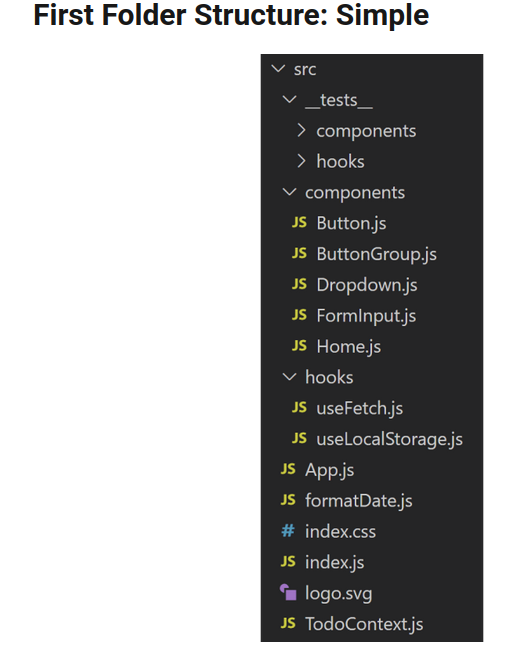
\includegraphics[width=9cm]{Develop/Languages/JavaScript/Frameworks/React/images/FoldersSimpleReact.png}
  \end{minipage}
\end{figure}


In the beginning, when you run the create-react-app, there are no folders in the src folder. Most people create a components folder and a hooks folder as their first two folders. Now, this is a very simple folder structure, it's not a bad way to do things for smaller projects with less than 10-15 components.
Hooks

Every custom hook in your project is stored in the hooks folder. This folder is useful for any size project because almost every project has more than one custom hook, and having a place to put them all can be extremely helpful.
Components

Since every component in your entire application will be contained in the components folder, the simple folder structure, it is very easy to understand. Since this folder can become very difficult to manage as your project grows beyond 10-15 components, our components are dispersed across multiple folders and given more structure in all other folder structures. However, for small projects, a single folder will do just fine without this extra complexity.
tests

This structure's final folder, the tests folder, contains all of your test code. Typically, We can discover that people keep all of their tests in a single folder for smaller projects like this one (that is if they write any tests at all). Overall, We tend to believe this is fine for smaller projects, but as your project gets bigger, the recommendation would be to change this.
Advantages

We can conclude that the most important advantage of this folder structure is its simplicity, but the structure is not that much functional beyond that.
Disadvantages

You'll observe that this folder structure leaves it up to the user to decide what to do with objects like photos, utility functions, React contexts, etc. The reason is that you can get away with merely placing those files in the root of your src folder as smaller projects typically don't have as many of these extra files. Any project larger than a small project should use at least an intermediate folder structure because it will become a mess quickly as your project grows.

\subsection{Segunda estructura de carpertas: Intermedio}

\begin{figure}[h!]
  \center
  \begin{minipage}{5cm}
    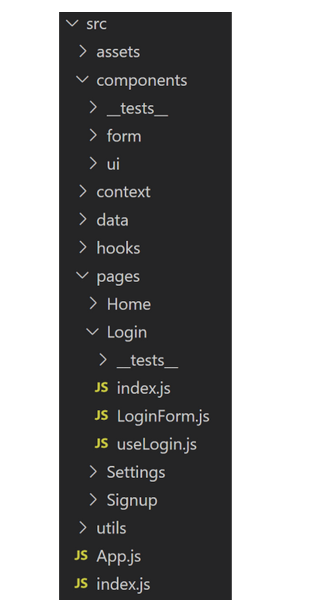
\includegraphics[width=4cm]{Develop/Languages/JavaScript/Frameworks/React/images/FolderIntermedioReact.png}
  \end{minipage}
\end{figure}

As you can see from the image above, this folder structure has a ton more folders that cover just about any file type you could imagine in a React project. With a folder layout like this, you should primarily only have files like your index.js file in the root of your src folder.

The fact that we are now segmenting our project into pages, which contain all the logic for specific pages in a single location, is the other significant difference between this folder structure and the simple folder structure. The ability to find all the data related to your pages in one folder rather than having to search through multiple folders and sift through irrelevant files is really helpful when working on larger projects.

Additionally, you'll see that our tests are now tailored to the particular folder and files they are testing. This makes it simpler to identify the code that has been tested, which in turn makes testing code easier in general when tests are positioned next to the code that is being tested.
Pages

The addition of the pages folder represents the most significant change to this folder structure. Each page of your application should have its own folder in this location. There should be a single root file for your page (usually index.js) and all the files that are specific to that page inside of those page-specific folders. For instance, the Login page in the image above has the root file index.js, the LoginForm component, and a unique hook called useLogin. Since the Login page is the only place that the component and hook are ever used, they are stored with this page rather than in the global hooks or components folders.

The main advantage of this system over the previous (simple) folder structure is the separation of page-specific code from your more general global code. When all of the pertinent code is centralized in a single folder, it is simpler to understand what your application is doing.
Components

Another significant difference in this example is the further subdivision of our components folder into subfolders. These subfolders are quite helpful since they keep your components separated into different groups rather than just being a big blob of them. Our example includes a ui folder that contains all of our user interface elements, such as buttons, modals, cards, etc. For controls related to forms, such as checkboxes, inputs, date pickers, etc., we also have a form folder.

This components folder can be tailored and broken down anyway you see appropriate based on the requirements of your project, but in ideal circumstances, this folder shouldn't grow too large as many of your more intricate components will be kept in the pages folder.
Hooks

The hooks folder is the last folder that somehow repeats the simple folder structure. This folder is nearly comparable to the previous hooks folder, but it only stores global hooks that are used across several pages, not every hook in your application. This is due to the fact that the pages folder houses all page-specific hooks.
Assets

All of the project's photos, CSS files, font files, etc. are located under the assets folder. All that isn't related to coding will be kept in this folder.
Context

All of your React context files used on lots of pages are kept in the context folder. Having a single folder to put them in is particularly helpful when working on larger projects because you will likely utilize several contexts throughout your application. You can swap out this folder with a better collection of folders for storing Redux files if you're using a different global data store, like Redux.
Data

Comparable to the assets folder, the data folder is used to house our data assets, such as JSON files that contain information used in our programs (store items, theme information, etc). Additionally, a file containing global constant variables may be kept in this subdirectory. This is helpful if your program uses a lot of constants, such as environment variables.
Utils

The utils folder is the last new folder that we have in this type of structuring. To store all utility features, including formatters, use this folder. This folder is rather simple, and all of the files inside of it ought to be simple as well. Since a utility function with side effects is probably not just a straightforward utility function, I prefer to only place pure functions in this subdirectory. Of course, there are exceptions to any rule.
Advantages

The fact that each of your files has its own folder is the main advantage of this new approach. There should be almost no files in the root src folder.

Your files are now collocated according to the page they are used in, which is another enormous advantage. This is advantageous since it generally makes understanding, writing, and reading code easier and decreases the amount of global code kept in your general components, hooks, etc. directories. As a project expands, it becomes more and more crucial to have files that are used together stored together.
Disadvantages

The greatest disadvantage of this method is that your pages folder will start to lose value as your application gets bigger and bigger. This is because it is increasingly likely that a single feature will be used across numerous pages rather than simply one when your application obtains more pages. This reduces the use of your pages folder and bloats your other files because you have to relocate the code out of the pages folder and into the other folders in your program.

The pages folder for your to-do page can house all the code for your to-dos, for instance, if your simple to-do list application only keeps track of your tasks on one page. You can no longer retain these to-do files in your pages folder if you later create a second page that allows you to categorize your to-dos under projects. This is because you now have two pages that must display to-do information. Nearly all of your code will be shared over numerous pages until your site reaches a certain size, which is where the sophisticated folder structure comes in.


\subsection{Tercera estructura de carpertas: avanzado}

\begin{figure}[h]
  \center
  \begin{minipage}{5cm}
    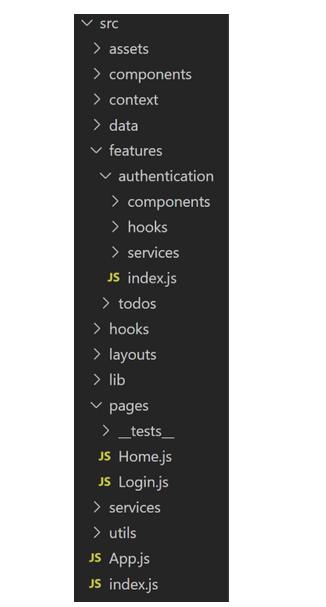
\includegraphics[width=4cm]{Develop/Languages/JavaScript/Frameworks/React/images/FolderAvantageReact.png}
  \end{minipage}
\end{figure}



Tomado de un art\'iculo  \href{https://dev.to/fpaghar/folder-structuring-techniques-for-beginner-to-advanced-react-projects-30d7}{\blue Dev}


?`Qu\'e es una SPA?

\section{Hooks}
Los hooks son una nueva caracter\'istica en React 16.8. Estos me permiten usar el estado y otras caracteristicas de React sin escribir un clase.

Los hooks resuelven una amplia variedad de problemas aparentemente desconectados en React que hemos encontrado durante m\'as de conco a\~nos de escribir
mantener decenas de miles de componentes.

Esta secc\'on es tomada de \href{https://es.reactjs.org/docs/hooks-intro.html}{\blue Documentaci\'on de React}

En lo siguiente veremos unos tantos hooks.
\subsection{useState}
\begin{itemize}
    \item Use a state variable when a component needs to ``remember'' some information between renders.
    \item State variables are declared by calling the useState Hook.
    \item Hooks are special functions that start with use. They let you ``hook into'' React features like state.
    \item Hooks might remind you of imports: they need to be called unconditionally. Calling Hooks, including useState, is only valid at the top level of a component or another Hook.
    \item The useState Hook returns a pair of values: the current state and the function to update it.
    \item You can have more than one state variable. Internally, React matches them up by their order.
    \item State is private to the component. If you render it in two places, each copy gets its own state.
\end{itemize}

\begin{verbatim}
    import { useState } from 'react';
    import { sculptureList } from './data.js';
    
    export default function Gallery() {
      const [index, setIndex] = useState(0);
      const [showMore, setShowMore] = useState(false);
    
      function handleNextClick() {
        setIndex(index + 1);
      }
    
      function handleMoreClick() {
        setShowMore(!showMore);
      }
    
      let sculpture = sculptureList[index];
      return (
        <>
          <button onClick={handleNextClick}>
            Next
          </button>
          <h2>
            <i>{sculpture.name} </i> 
            by {sculpture.artist}
          </h2>
          <h3>  
            ({index + 1} of {sculptureList.length})
          </h3>
          <button onClick={handleMoreClick}>
            {showMore ? 'Hide' : 'Show'} details
          </button>
          {showMore && <p>{sculpture.description}</p>}
          <img 
            src={sculpture.url} 
            alt={sculpture.alt}
          />
        </>
      );
    }
\end{verbatim}
\begin{verbatim}


  export const sculptureList = [{
  name: 'Homenaje a la Neurocirugía',
  artist: 'Marta Colvin Andrade',
  description: 'Although Colvin is predominantly known for 
                abstract themes that allude to pre-Hispanic symbols, 
                this gigantic sculpture, an homage to neurosurgery, 
                is one of her most recognizable public art pieces.',
  url: 'https://i.imgur.com/Mx7dA2Y.jpg',
  alt: 'A bronze statue of two crossed hands delicately holding a human
        brain in their fingertips.'  
}, {
  name: 'Floralis Genérica',
  artist: 'Eduardo Catalano',
  description: 'This enormous (75 ft. or 23m) silver flower is located in
                Buenos Aires. It is designed to move, closing its petals in 
                the evening or when strong winds blow and opening them 
                in the morning.',
  url: 'https://i.imgur.com/ZF6s192m.jpg',
  alt: 'A gigantic metallic flower sculpture with reflective 
        mirror-like petals and strong stamens.'
}, {
  name: 'Eternal Presence',
  artist: 'John Woodrow Wilson',
  description: 'Wilson was known for his preoccupation with equality, 
                social justice, as well as the essential and spiritual 
                qualities of humankind. This massive (7ft. or 2,13m) 
                bronze represents what he described as "a symbolic Black 
                presence infused with a sense of universal humanity."',
  url: 'https://i.imgur.com/aTtVpES.jpg',
  alt: 'The sculpture depicting a human head seems ever-present and solemn. 
        It radiates calm and serenity.'
}, {
  name: 'Moai',
  artist: 'Unknown Artist',
  description: 'Located on the Easter Island, there are 1,000 moai, or extant
                 monumental statues, created by the early Rapa Nui people, 
                 which some believe represented deified ancestors.',
  url: 'https://i.imgur.com/RCwLEoQm.jpg',
  alt: 'Three monumental stone busts with the heads that are disproportionately 
        large with somber faces.'
}, {
  name: 'Blue Nana',
  artist: 'Niki de Saint Phalle',
  description: 'The Nanas are triumphant creatures, symbols of femininity and 
                maternity. Initially, Saint Phalle used fabric and found 
                objects for the Nanas, and later on introduced polyester to 
                achieve a more vibrant effect.',
  url: 'https://i.imgur.com/Sd1AgUOm.jpg',
  alt: 'A large mosaic sculpture of a whimsical dancing female figure in a 
        colorful costume emanating joy.'
}, {
  name: 'Ultimate Form',
  artist: 'Barbara Hepworth',
  description: 'This abstract bronze sculpture is a part of The Family of Man 
                series located at Yorkshire Sculpture Park. Hepworth chose not to 
                create literal representations of the world but developed abstract
                 forms inspired by people and landscapes.',
  url: 'https://i.imgur.com/2heNQDcm.jpg',
  alt: 'A tall sculpture made of three elements stacked on each other reminding 
        of a human figure.'
}, {
  name: 'Cavaliere',
  artist: 'Lamidi Olonade Fakeye',
  description: "Descended from four generations of woodcarvers, Fakeye's work 
                blended traditional and contemporary Yoruba themes.",
  url: 'https://i.imgur.com/wIdGuZwm.png',
  alt: 'An intricate wood sculpture of a warrior with a focused face on a horse 
        adorned with patterns.'
}, {
  name: 'Big Bellies',
  artist: 'Alina Szapocznikow',
  description: "Szapocznikow is known for her sculptures of the fragmented body 
                as a metaphor for the fragility and impermanence of youth and
                 beauty. This sculpture depicts two very realistic large bellies 
                 stacked on top of each other, each around five feet (1,5m) tall.",
  url: 'https://i.imgur.com/AlHTAdDm.jpg',
  alt: 'The sculpture reminds a cascade of folds, quite different from bellies in
         classical sculptures.'
}, {
  name: 'Terracotta Army',
  artist: 'Unknown Artist',
  description: 'The Terracotta Army is a collection of terracotta sculptures 
                depicting the armies of Qin Shi Huang, the first Emperor of China. 
                The army consisted of more than 8,000 soldiers, 130 chariots with 
                520 horses, and 150 cavalry horses.',
  url: 'https://i.imgur.com/HMFmH6m.jpg',
  alt: '12 terracotta sculptures of solemn warriors, each with a unique facial
        expression and armor.'
}, {
  name: 'Lunar Landscape',
  artist: 'Louise Nevelson',
  description: 'Nevelson was known for scavenging objects from New York City debris, 
                which she would later assemble into monumental constructions. 
                In this one, she used disparate parts like a bedpost, juggling pin,
                 and seat fragment, nailing and gluing them into boxes that reflect 
                 the influence of Cubism's geometric abstraction of space and form.',
  url: 'https://i.imgur.com/rN7hY6om.jpg',
  alt: 'A black matte sculpture where the individual elements are initially 
        indistinguishable.'
}, {
  name: 'Aureole',
  artist: 'Ranjani Shettar',
  description: 'Shettar merges the traditional and the modern, the natural and the 
                industrial. Her art focuses on the relationship between man and 
                nature. Her work was described as compelling both abstractly and 
                figuratively, gravity defying, and a "fine synthesis of unlikely 
                materials."',
  url: 'https://i.imgur.com/okTpbHhm.jpg',
  alt: 'A pale wire-like sculpture mounted on concrete wall and descending on the 
        floor. It appears light.'
}, {
  name: 'Hippos',
  artist: 'Taipei Zoo',
  description: 'The Taipei Zoo commissioned a Hippo Square featuring submerged 
                hippos at play.',
  url: 'https://i.imgur.com/6o5Vuyu.jpg',
  alt: 'A group of bronze hippo sculptures emerging from the sett sidewalk as if 
        they were swimming.'
}];

    \end{verbatim} 
\subsection{useContext}
\href{https://dmitripavlutin.com/react-context-and-usecontext/}{useContext}

\subsection{useRef}

useRef es un React hook que te permite hacer referencia a un valor que no es necesario para renderizar.

Le aplica una referencia a los elemetos del DOM de JavaScript, que nos permite editar los estilos, lo m\'etodos entre otras propiedades.
Mod\'ifica y no realiza ningun render nuevo.


\subsection{useMemo}

Es un hooks de React que te permite guardar en cach\'e el resultado de un c\'alculo entre renderizados. 

\begin{lstlisting}
    const cachedValue = useMemo(calculateValue, dependencies);
\end{lstlisting}

{\Large\bf Referencia}

Se llama a useMemo en el nivel superior de tu compoente para guardar en cach\'e un c\'alculo entre rerenderizados: 

{\normalsize\bf Par\'ametros}


\begin{itemize}
    \item[calcularValor: ] la funci\'on que calcula el valor que deseas memorizar. Debe ser pura, no debe acerptar argumentos y debe devolver un valor de cualquier tipo. React llamar\'a a tu funci\'on durante el renderizado inicial. 
    En renderizados posteriores, React devolver\'a el mismo valor nuevamente si las dependecias no han cambiado desde el \'utimo renderizado. De lo contrario, llamar\'a a calcularValor, devolver\'a su resultado y lo almacenar\'a en caso de que pueda reutilizarse m\'as tarde.
    \item[dependecias: ] la lista de todos los valores reactivos a los que se hace referencia dentro del c\'odigo calcularValor. Los valores reactivos incluyen props, estado y todas las variables y funciones declaradas directamente dentro del cuerpo de tu componente. Si tu linter
\end{itemize}


\subsection{useInterval}


\section{react-router-dom}

\subsection{Enrutamiento del lado del cliente}

React router, es una librería que nos permite actualizar la URL desde un clic sin realizar una solicitud
de otro documento desde el servidor, esto permite mostrar inmediatamente una nueva interfaz de usuario y realizar solicitudes
de datos con b\'usqueda para actualizar la p\'agina con nueva informaci\'on.

Esto permite experiencias de usuario m\'as r\'apidas porque el navegador no necesita solicitar un documento
completamente nuevo o volver a evaluar los activos de CSS y JavaScript para sigueinte p\'agina. Tambi\'en permite experiencias de usuario m\'as din\'amizas
con cosas como la animaci\'on.

\subsection{Rutas anidadas}
El enrutamiento anidado es la idea general de acoplar segmentos de URL a la jerarqu\'ia y los datos de los componentes. Las rutas anidadas de React
Router se inspiraron en el sistema de enrutamiento de Ember.js alrededor de 2014. El equipo de Ember se dio cuenta de que, en casi todos los casos, los segmentos de la URL determinan:
\begin{itemize}
  \item Los dise\~nos para presentar en la p\'agina.
  \item Las dependencias de datos de esos dise\~nos.
\end{itemize}

React Router adopta est\'a convenci\'on con API para crear dise\~nos anidados acoplados a segmentos de URL y datos.


\subsection{Segmentos din\'amicos}

Se utiliza el hooks useParams de React-Router-Dom el cu\'al se utiliza para capturar los parametros en la URL en los componentes,
por ejemplo,
\begin{verbatim}
  <Route  exact path="/usuario/:username/:age"  element={<Usuario />} />
\end{verbatim}
En la componente usuario si se invoca el useParams se obtiene un objeto
\begin{verbatim}
  {
    username:"Nombre_especificado_Url",
    age:"Edad_especificada"
  }
\end{verbatim}